\section{Results}
\begin{figure}[h]
	\begin{center}
		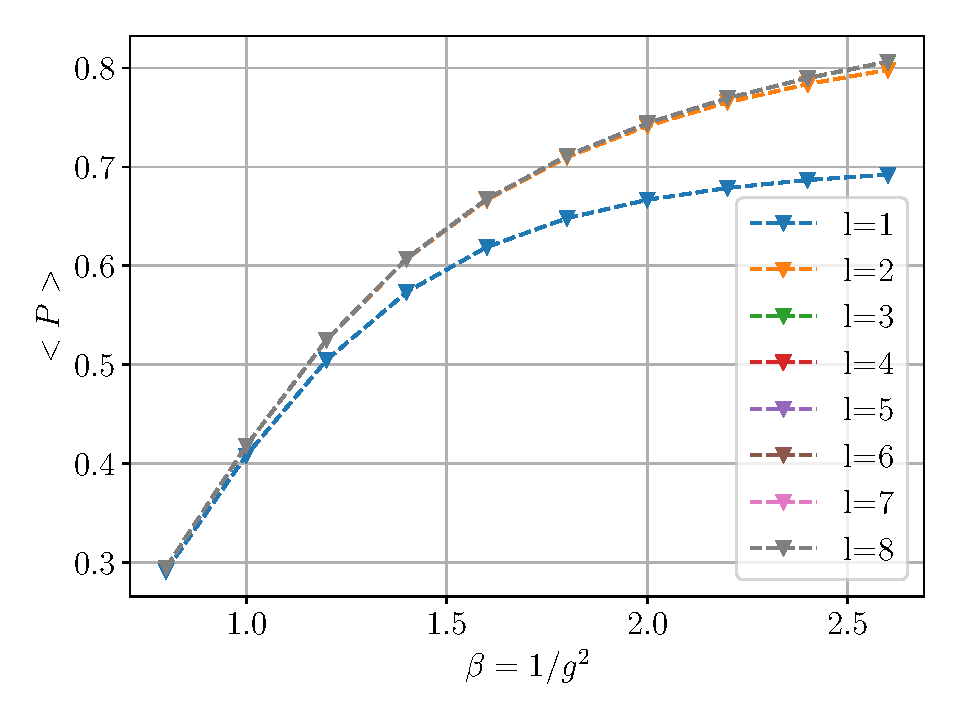
\includegraphics[width=0.45\textwidth]{images/PlaquetteExp2x2.pdf}
	\end{center}
	\caption{plaquette expectation values for a 2x2 lattice.}
\end{figure}
\begin{figure}[h]
	\begin{center}
		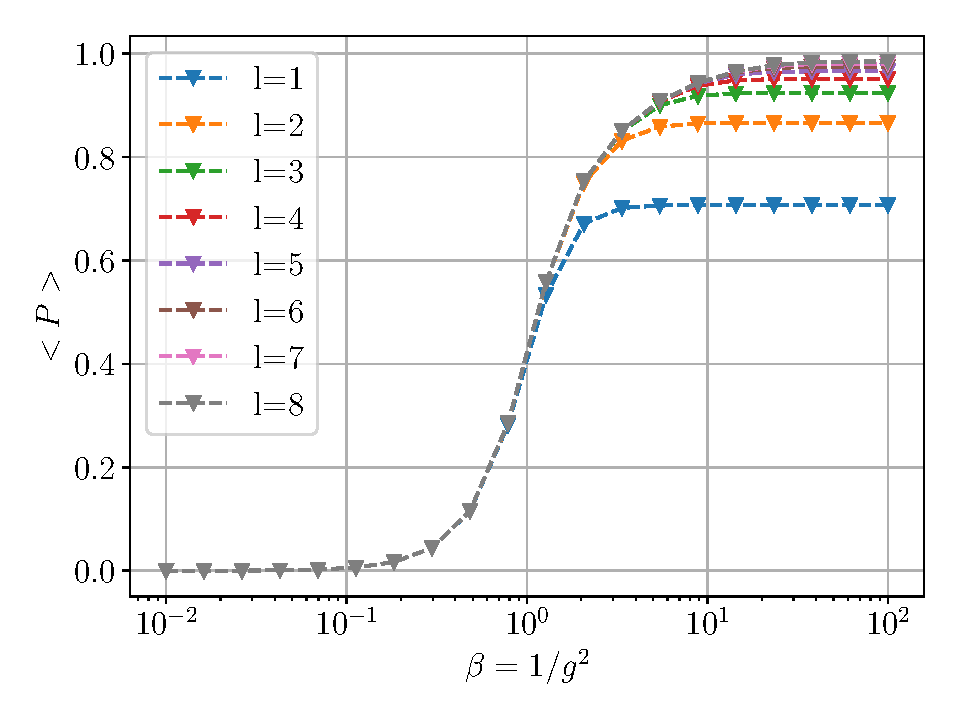
\includegraphics[width=0.45\textwidth]{images/PlaquetteExp2x2Log.pdf}
	\end{center}
	\caption{Plaquette expectation values for a 2x2 lattice in a logarithmic plot.}
\end{figure}
\begin{figure}[h]
	\begin{center}
		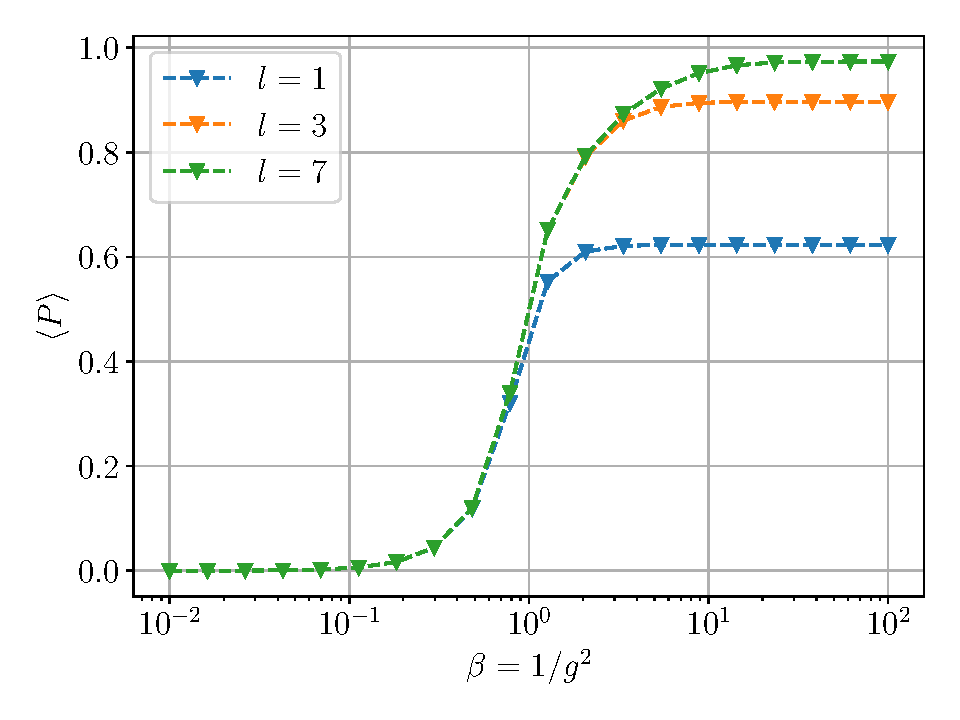
\includegraphics[width=0.45\textwidth]{images/PlaquetteExp2x2PBC.pdf}
	\end{center}
	\caption{plaquette expectation values for a 2x2 pbc lattice.}
\end{figure}
\begin{figure}[h]
	\begin{center}
		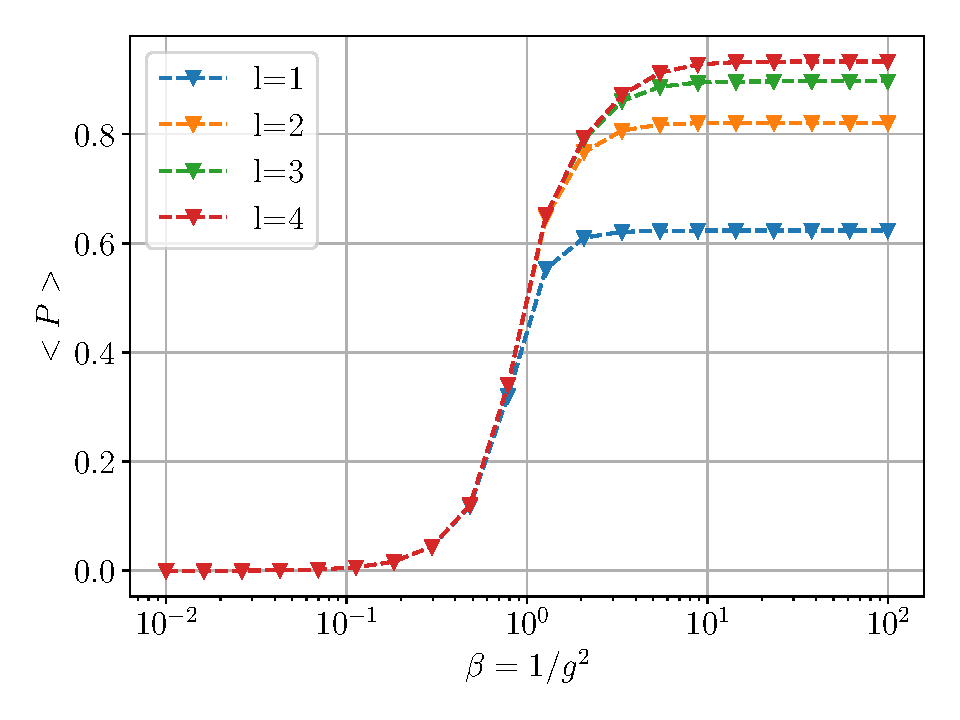
\includegraphics[width=0.45\textwidth]{images/PlaquetteExp2x2PBCLog.pdf}
	\end{center}
	\caption{Plaquette expectation values for a 2x2 pbc lattice in a logarithmic plot.}
\end{figure}
\begin{figure}[h]
	\begin{center}
		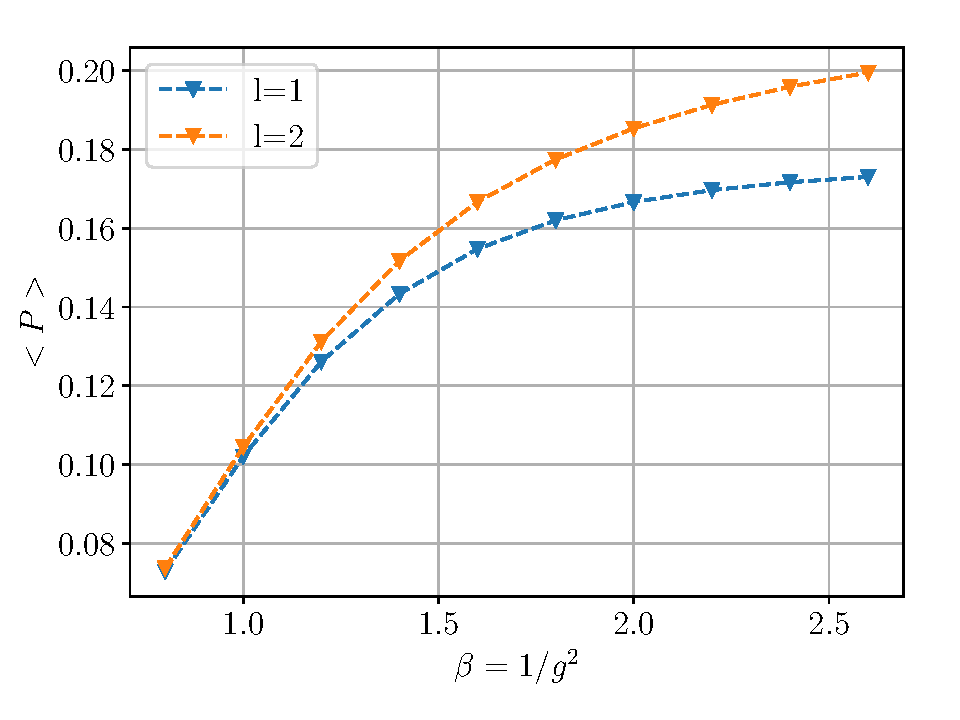
\includegraphics[width=0.45\textwidth]{images/PlaquetteExp3x3.pdf}
	\end{center}
	\caption{Plaquette expectation values for a 3x3 lattice.}
\end{figure}
\begin{figure}[h]
	\begin{center}
		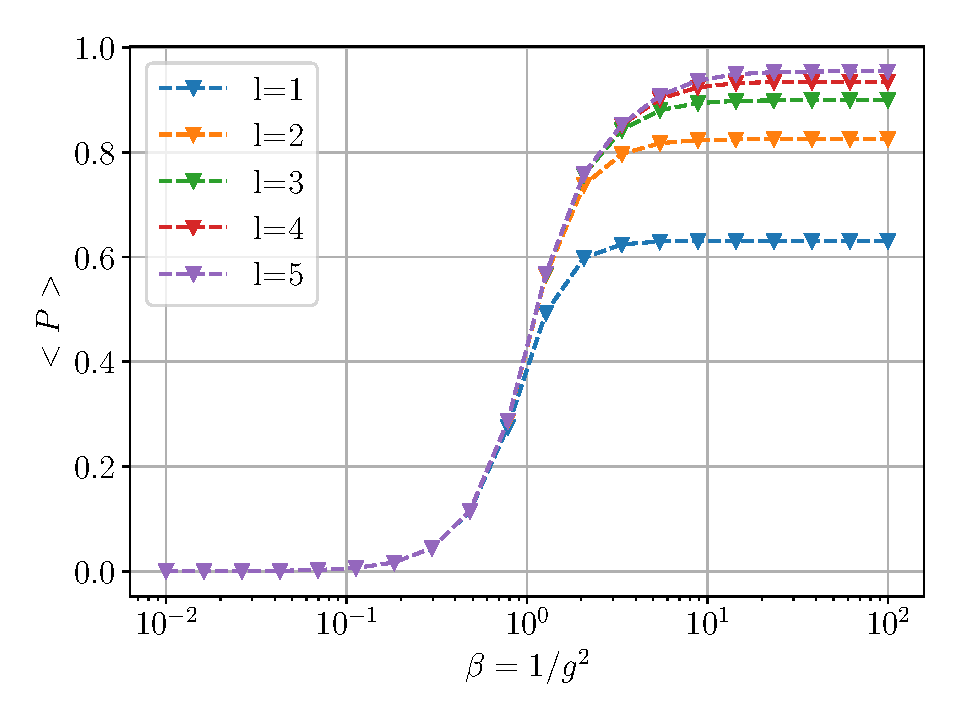
\includegraphics[width=0.45\textwidth]{images/PlaquetteExp3x3Log.pdf}
	\end{center}
	\caption{Plaquette expectation values for a 3x3 lattice in a logarithmic plot.}
\end{figure}
\begin{figure}[h]
	\begin{center}
		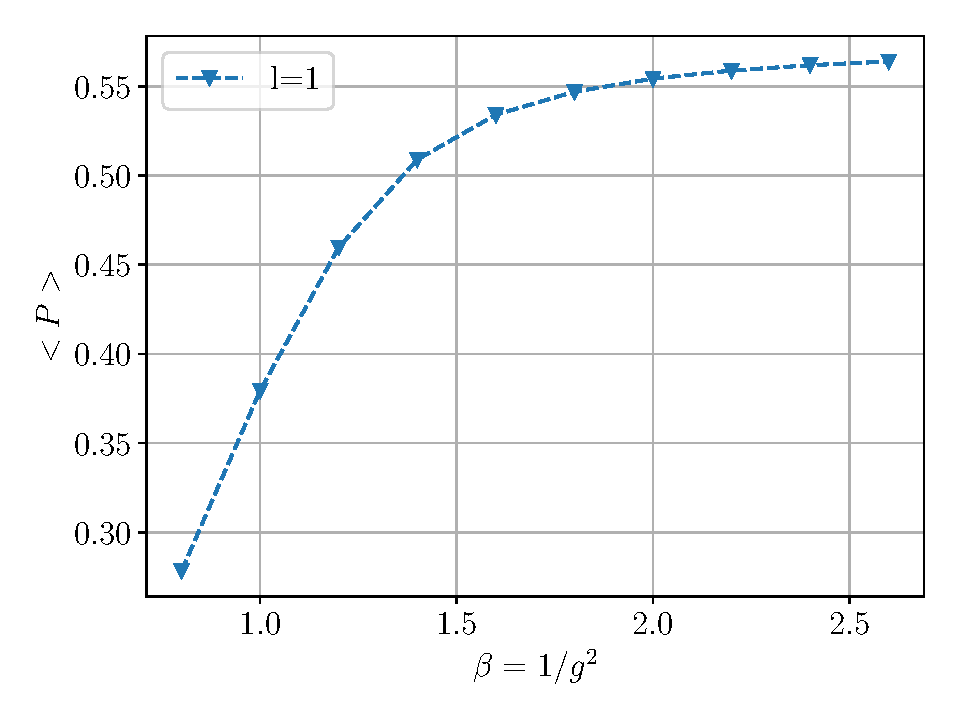
\includegraphics[width=0.45\textwidth]{images/PlaquetteExp3x3PBC.pdf}
	\end{center}
	\caption{Plaquette expectation values for a 3x3 pbc lattice.}
\end{figure}
\begin{figure}[h]
	\begin{center}
		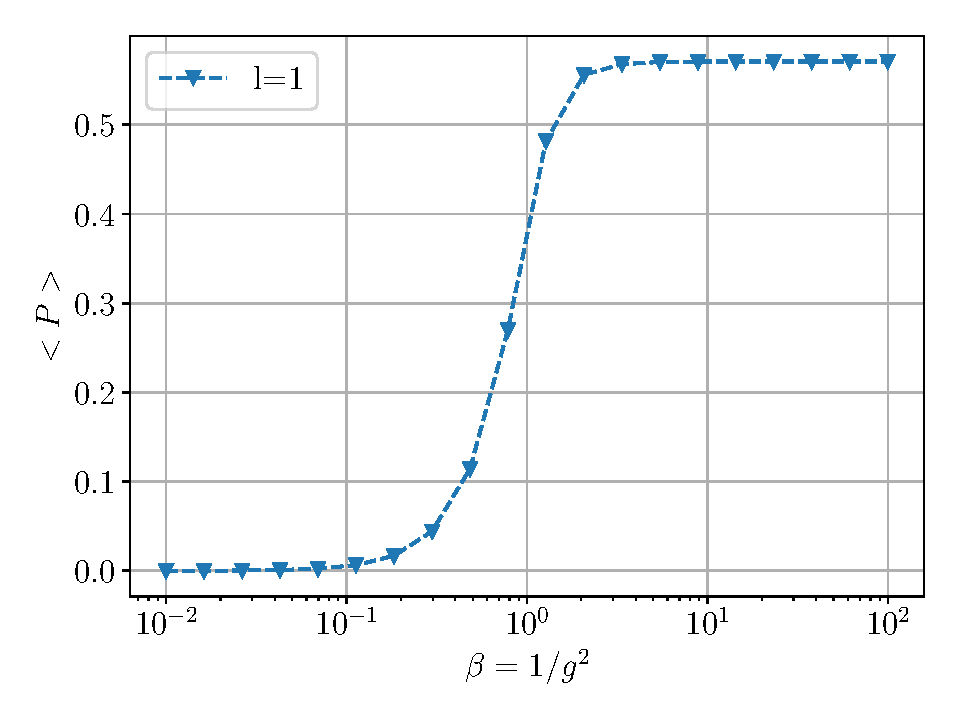
\includegraphics[width=0.45\textwidth]{images/PlaquetteExp3x3PBCLog.pdf}
	\end{center}
	\caption{Plaquette expectation values for a 3x3 pbc lattice in a logarithmic plot.}
\end{figure}
\newpage
fds
\begin{figure}[h]
	\begin{center}
		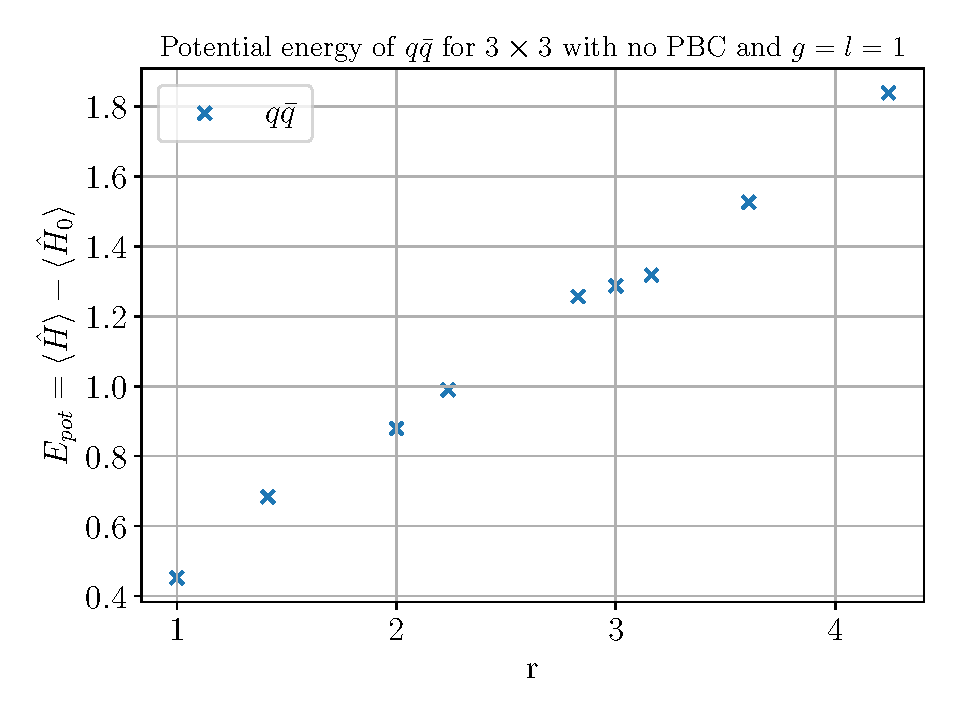
\includegraphics[width=0.45\textwidth]{images/quark-antiquark-potential.pdf}
	\end{center}
	\caption{Quark-Antiquark potential.}
\end{figure}
\begin{figure}[h]
	\begin{center}
		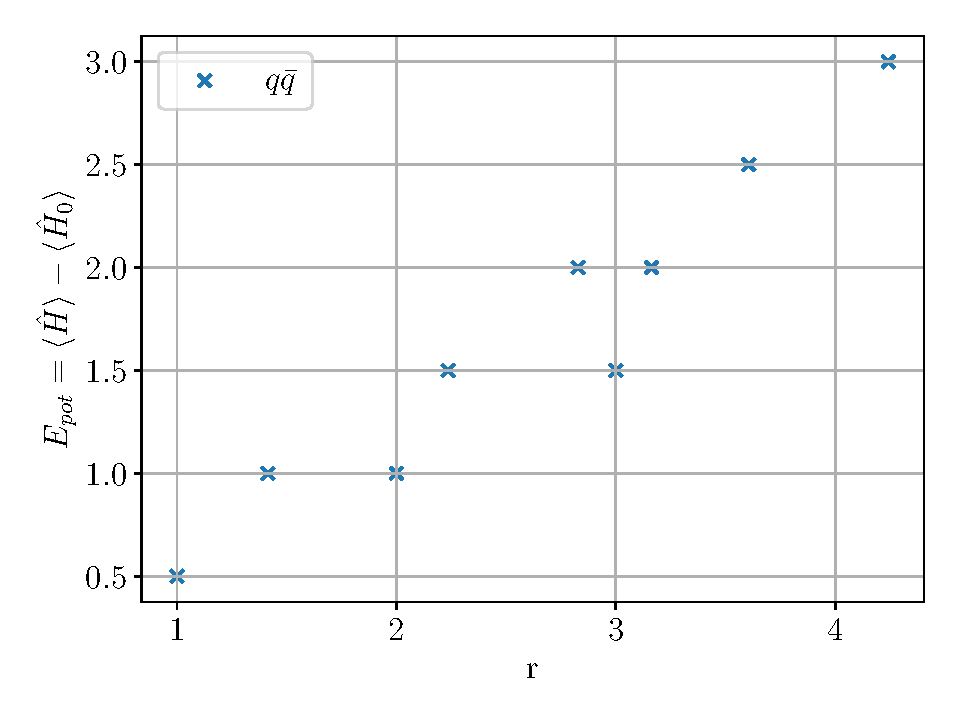
\includegraphics[width=0.45\textwidth]{images/quark-antiquark-potential2.pdf}
	\end{center}
	\caption{Quark-Antiquark potential for 4x4 lattice with l=g=1.}
\end{figure}

\begin{figure}[h]
	\begin{center}
		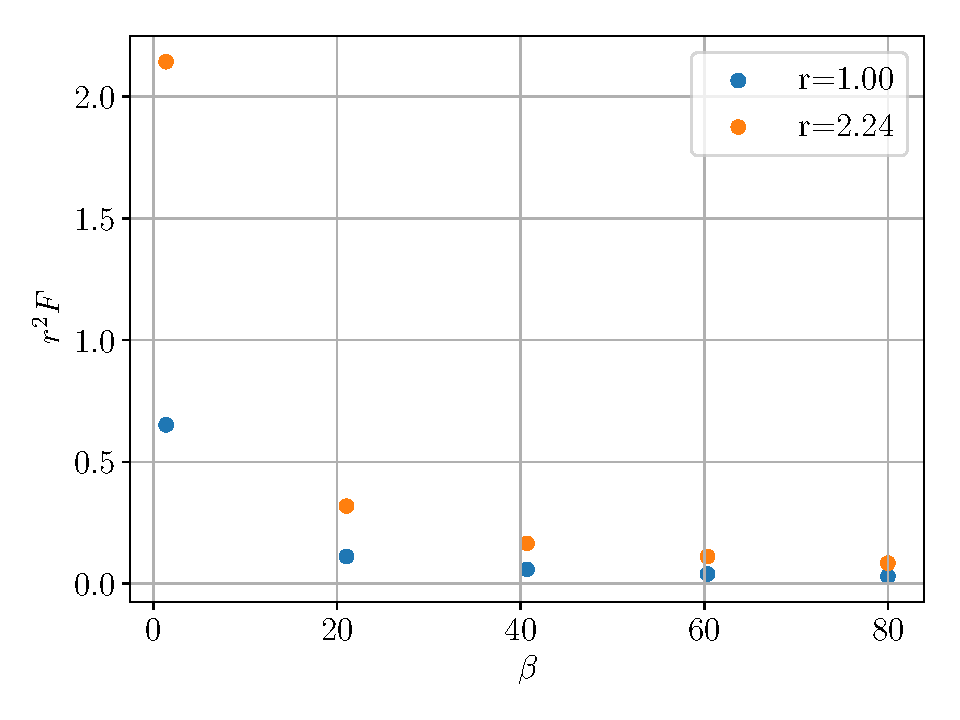
\includegraphics[width=0.45\textwidth]{images/step_scaling.pdf}
	\end{center}
	\caption{Quark-Antiquark potential.}
\end{figure}
